\documentclass[a4paper]{report}
\pagestyle{headings}
\usepackage{hyperref}
\usepackage{listings}
\usepackage{graphicx}
\lstset{language=bash}
\lstset{numbers=right}
\lstset{breaklines}
\title{Lab Report for Object-oriented Programming course \newline
 Lab 2: Preprocessor}
\author{Wang, Chen \\ 16307110064 \\ School of Software\\ Fudan University}
\date{\today}
\bibliographystyle{plain}
\begin{document}
\maketitle

\tableofcontents

\chapter{Background Knowledge \& Concepts Required for This Lab}
\section{C/C++ Compiling Process}

\subsection{Overall process of compiling}

\subsection{Preprocessing}


\subsection{Parsing}

\subsection{Global Optimization}


\subsection{Code Generation}
\subsection{Peehole Optimization}
\subsection{Linking}
\section{C/C++ Preprocessing}

\subsection{The need of preprocessing}


\subsection{Different preprocessing algorithms}


\subsection{Preprocessing algorithm utilized by the current g++}

\subsection{Encapsulation}

\chapter{Specifications of This Lab}
\section{Regulations in the preprocessing process}

\section{Test cases designed in the lab}


\section{Other specifications of the programming}

\chapter{Structure and  the OO Ideas Adopted}
\section{Objected-oriented ideas adopted in the implementation}
\subsection{Encapsulation}


\chapter{Running Result of My Implementation}
The following screenshots are the tests that are identical to the steps in the requirement documentation and proves that my version of implementation functions identical to the standard version.
\section{The first sample test}
The results are shown as Figure \ref{2}. 

\begin{figure}
  \centering
  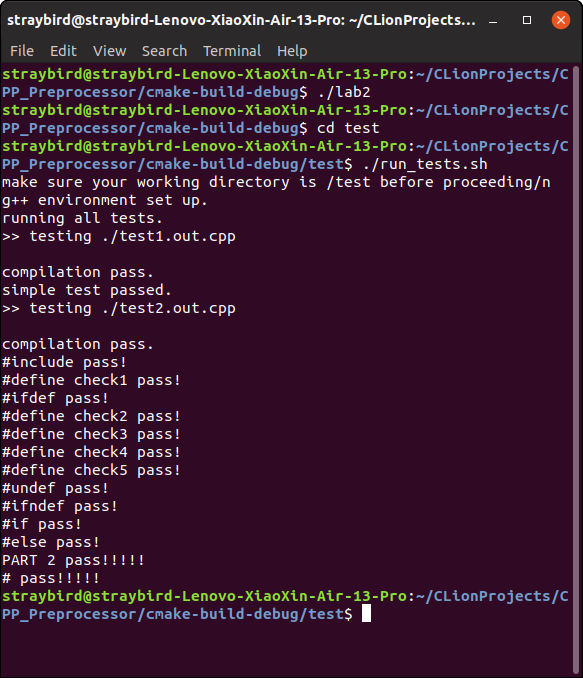
\includegraphics[width=12cm]{shell.png}
  \caption{Testcase Result}\label{2}
\end{figure}

\begin{figure}
  \centering
  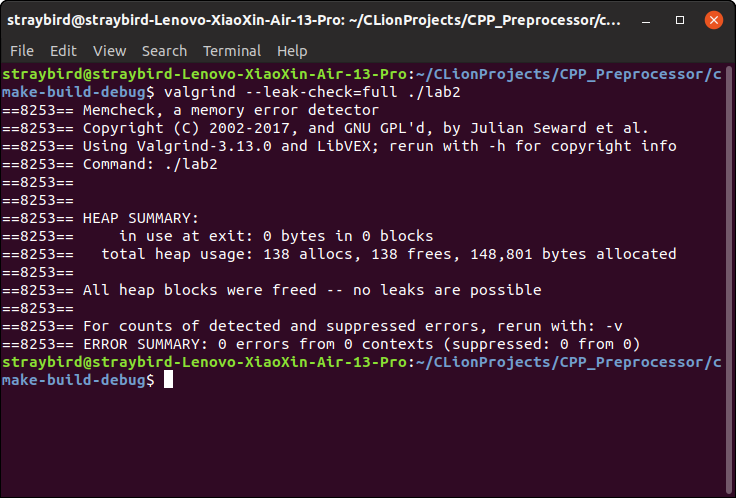
\includegraphics[width=12cm]{mem.png}
  \caption{Memory Leak Check}\label{2}
\end{figure}
\begin{thebibliography}{A}

\bibitem{1}
Wikipedia contributors. (2019, February 3). Encapsulation (computer programming). In \emph{Wikipedia, The Free Encyclopedia}. Retrieved 10:19, March 23, 2019, from \url{https://en.wikipedia.org/w/index.php?title=Encapsulation_(computer_programming)&oldid=881507936}

\bibitem{2}
Wikipedia contributors. (2019, March 17). Reversi. In \emph{Wikipedia, The Free Encyclopedia}. Retrieved 10:20, March 23, 2019, from \url{https://en.wikipedia.org/w/index.php?title=Reversi&oldid=888167585}

\bibitem{3}
Wikipedia contributors. (2019, March 15). Polymorphism (computer science). In \emph{Wikipedia, The Free Encyclopedia}. Retrieved 10:21, March 23, 2019, from \url{https://en.wikipedia.org/w/index.php?title=Polymorphism_(computer_science)&oldid=887878749}

\bibitem{4}
Wikipedia contributors. (2019, February 27). Object-oriented programming. In \emph{Wikipedia, The Free Encyclopedia}. Retrieved 10:22, March 23, 2019, from \url{https://en.wikipedia.org/w/index.php?title=Object-oriented_programming&oldid=885274966}

\bibitem{5}
Wikipedia contributors. (2019, February 21). Inheritance (object-oriented programming). In \emph{Wikipedia, The Free Encyclopedia}. Retrieved 10:22, March 23, 2019, from \url{https://en.wikipedia.org/w/index.php?title=Inheritance_(object-oriented_programming)&oldid=884436146}

\end{thebibliography}
\end{document} 